%Correct the file name.
%X: book number
%Y: part number
%ZZZ: page number in three digits. So page 3 would be 003.

\documentclass[11pt]{amsbook}

\usepackage{../HBSuerDemir}	% ------------------------


\begin{document}

% ++++++++++++++++++++++++++++++++++++++
\hPage{feyzioglu-081}
% ++++++++++++++++++++++++++++++++++++++
\begin{lem}

\noindent$a_1,a_2, \dotsc ,a_n \in G$. Then the products of $a_1,a_2, \dots ,a_n$ are independent of the mode of putting parantheses. This means the following. We define

\begin{flalign*}
P_1(a_1) &= \{a_1\} \\
P_2(a_1,a_2) &= \{a_1a_2\} \\
P_3(a_1,a_2,a_3) &= \{(a_1a_2)a_3,a_1(a_2a_3)\} \\
&=\{xy: x \in P_1(a_1), y \in P_2(a_2,a_3) \quad \textrm{or} \quad x \in P_2(a_1,a_2), y \in P_1(a_3)\} \\
P_4(a_1,a_2,a_3,a_4) &= \{a_1(a_2(a_3a_4),a_1((a_2,a_3)a_4), ((a_1a_2)a_3)a_4, (a_1(a_2a_3))a_4\} \\
&=\{xy: x \in P_1(a_1), y \in P_3(a_2,a_3,a_4) \quad \textrm{or} \\
&\quad x \in P_2(a_1,a_2), y \in P_2(a_3.a_4) \quad \textrm{or} \\
&\quad x \in P_3(a_1,a_2,a_3), y \in P_1(a_4)\} 
\end{flalign*}
\[\dotsc \dotsc \dotsc \dotsc \dotsc \dotsc \dotsc \dotsc \dotsc \dotsc \dotsc \dotsc \dotsc \dotsc \dotsc \dotsc \dotsc\]
\[P_k(a_1,a_2,\dotsc,a_k) = \{ xy: x \in P_i(a_1,a_2,\dotsc,a_i), y \in P_{k-i}(a_{i+1},\dotsc,a_k) \quad \text{for some} \quad i = 1,2, \dotsc,k \}\]
\\
for $k = 1,2,\dotsc,n$. Thus $P_k$ are subsets of $G$ whose elements are the products of $a_1,a_2, \dots ,a_k$ reduced to $k-1$ successive multiplications of two elements in $G$.
\\
\\
Claim: For all $n \in \hSoN$ and for all $a_1,a_2, \dots ,a_n \in G$. the set $P_n(a_1,a_2,\dotsc,a_n)$ contains one and only one element.

\end{lem}

\begin{proof}
\noindent The proof will be the induction on $n$ (in the form 4.5). For $n = 1,2,$ it is evident that $P_1(a_1),P_2(a_1,a_2)$ each have exactly one element. For $n =3$, the claim is just the associativity of multiplication. For $n=4$, the argument preceding the lemma proves the claim. Notice that we used only the associativity of multiplication here.
\\
\\
Suppose $n \geq 5 $ and the lemma is proved for $1,2, \dots , n-1$. Let $u,v \in P_n(a_1,a_2,\dotsc,a_n)$. We are to prove $u=v$. By the definition of $P_n(a_1,a_2,\dotsc,a_n)$, we have $u = xy,$ $v=st$, where
\[x \in P_i(a_1,a_2,\dotsc,a_i), y \in P_{n-i}(a_{i+1},\dotsc,a_n), \quad  i \in \hSoN, \quad 1 \leq i \leq n-1,\]
\[s \in P_j(a_1,a_2,\dotsc,a_j), t \in P_{n-j}(a_{j+1},\dotsc,a_n), \quad  j \in \hSoN, \quad 1 \leq j \leq n-1,\]
\\
We prove $u=v$ first under the assumption $i=j$. By the induction, the set $P_i(a_1,a_2,\dotsc,a_i)$ contains one and only one element. Hence $x=s$. Also,
\end{proof}

% =======================================================
\end{document}  

%==== templates ====

%==== environments ====

%\begin{figure}[htb]
%	\centering
%	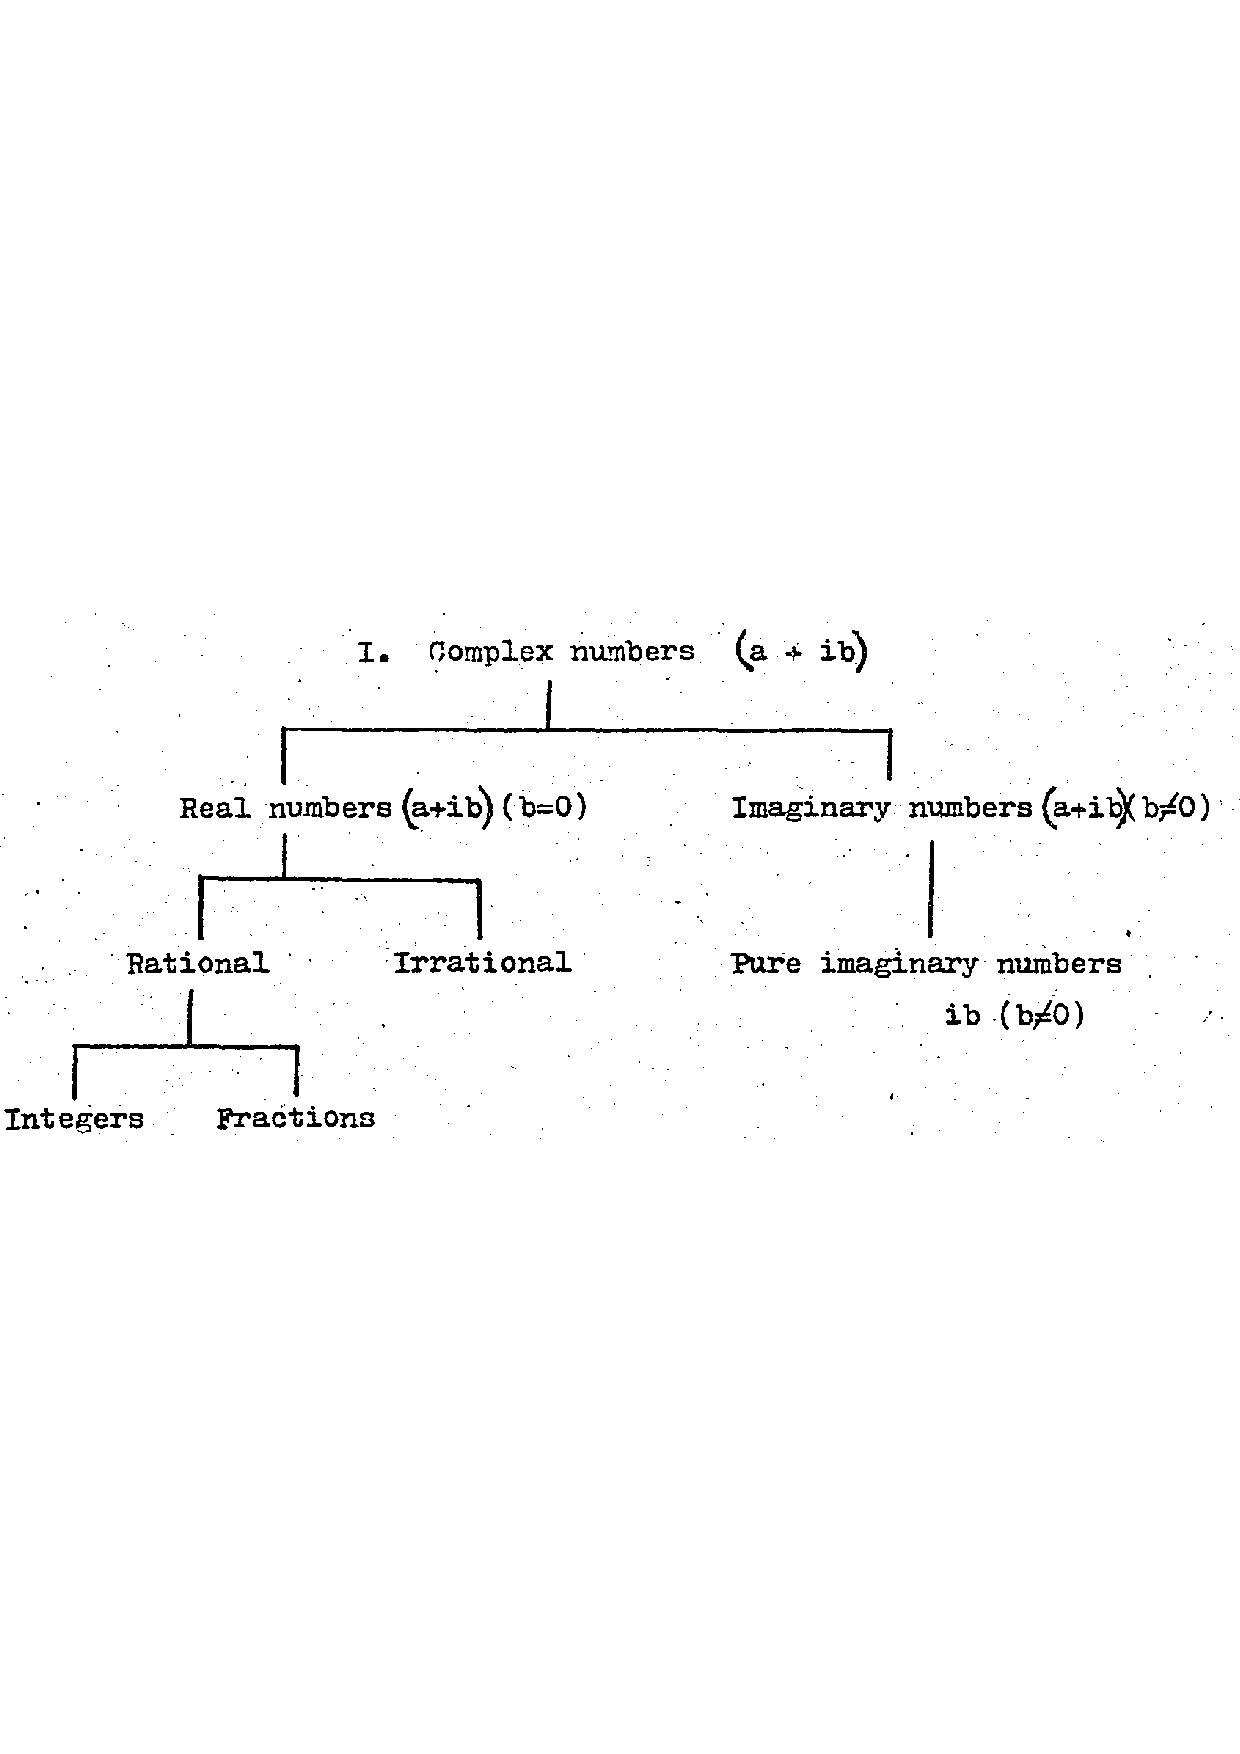
\includegraphics[width=0.9\textwidth]{images/SD-1-1p15A}
%	\caption{Classification of complex numbers}
%	\label{fig:classificationOfComplexNumbersA}
%\end{figure}

%\begin{center}
%\begin{tabular}{cc}
%\end{tabular}
%\end{center}

%\begin{exmp}
%\begin{hSolution}
%\end{hSolution}
%\end{exmp}

%\begin{hEnumerateAlpha}
%\end{hEnumerateAlpha}

%\begin{hEnumerateRoman}
%\end{hEnumerateRoman}

%$
%\begin{bmatrix}
%\end{bmatrix}
%$

%\frac{aaaa}{bbb}
%\frac{a_{n}}{b_{n}}
%\left( aaaa \right)
%\Longrightarrow

%\begin{multicols}{2}
%	bb
%\columnbreak
%	aa
%\end{multicols}
